\section{The steering engine}\label{sec:engine}

This chapter derives the on-chip engine that moves twenty or more tweezers independently along one row, compares it with the switched-port star coupler, and gives the beam-propagation design D1 with its simulated errors, power cost and limits.

\subsection{The requirement and what an AOD supplies}\label{sec:engine-req}

Section~\ref{sec:platform-opa} showed that the number of resolvable positions of an OPA along its steering axis equals its channel number $N$: 64 channels place at most about 15 tweezers on a row of 4~\textmu m sites, and more than 20 need 128 channels. Count alone is not the requirement, however. Rearrangement needs each tweezer to move on its own, as the tones of an acousto-optic deflector (AOD) do. An AOD owes this to two physical ingredients (standard AOD physics, [REF?] for a citable source): (i) frequency tagging, since each RF tone shifts its diffracted light by its own frequency, so that tweezers from different tones add incoherently on average and each tone's amplitude sets one tweezer's depth; and (ii) a time-delay medium, since the acoustic transit time across the aperture converts each tone's frequency into its own angle, and the number of resolvable spots is the RF bandwidth times the transit time. The independence is per axis. A single AOD moves its spots independently along one line, and crossed AODs give a grid of row and column tones rather than independent 2D positions (ref.~[17] of the proposal~\cite{proposal}). Hence the fair target for an integrated engine is a 1D AOD along a row.

A shared-arm OPA, in which every tweezer uses every arm, has neither ingredient, and phase-only synthesis couples all tweezers. We tested this directly on a 128-channel OPA with 20 synthesised tweezers. Removing one of them by warm-started re-synthesis (that site added to the dark points) leaves 1.9 to 3.3\% of the tweezer intensity at its site ($-15$ to $-17$~dB), changes the 19 kept tweezers by up to 12\%, and along a linear phase path between the two patterns the kept tweezers deviate by up to 19\%. Stray light at untargeted sites stays at about 2\%. Such an engine cannot gate 894.6~nm light at 50~dB, and it perturbs every other atom whenever one tweezer is switched.

Table~\ref{tab:engine-routes} lists the routes we considered for supplying an equivalent of at least one AOD ingredient. Route~E, the sliding-window focal-plane OPA, is the only one that works at a single optical frequency, uses only components already in the proposal (SiN star coupler, MZI trees, PZT or AlN shifters) and needs no new physics. Complex synthesis on the arms (A$'$) is a fallback with fewer optical elements, but needs amplitude modulation on every arm and power headroom, because moving one tweezer changes the optimum. The wavelength-addressed route (D) is excluded by the chromatic focal shift of a diffractive meta-objective unless that objective is made achromatic over several nanometres around 1064~nm.

\begin{table}[htbp]\centering\small
\caption{Routes to independently steered tweezers on one row (20 tweezers). Efficiencies are simulated (E, A$'$, F) or derived (D, G, T). The surface-acoustic-wave velocity used for route G ($\sim$5~km/s) is recalled, to be verified for an AlN/SiN/SiO$_2$ stack.}
\label{tab:engine-routes}
\begin{tabularx}{\linewidth}{@{}p{0.2\linewidth}Xp{0.13\linewidth}X@{}}
\toprule
Route & Source of independence & Efficiency & Show-stopper or cost \\
\midrule
E: sliding-window focal-plane OPA & tweezers on separate ports (position basis), linear superposition & 0.40 at centre, 0.19 at field edge & 127 fast splitters and 128 phase shifters; ${\sim}1\%$ per-port accuracy \\
A$'$: complex synthesis on the arms & linear superposition of 20 phase ramps (amplitude and phase per arm) & 0.75 (peak-to-mean 1.34) & 128 amplitude and phase modulators; power headroom \\
F: AOD emulation on the arms & one RF tone per tweezer: frequency tags and per-tone phase ramps & 0.44 (peak-to-mean 2.28) & 256 RF-driven modulators; intermodulation ghosts from modulator nonlinearity \\
D: wavelength-addressed dispersive OPA & optical frequency tags and delay lines & high (passive) & focal shift 14~\textmu m/nm allows only $\pm71$~pm ($\pm19$~GHz); 5~GHz per site needs 6.7~m of delay lines \\
G: integrated surface-acoustic-wave deflector & a literal AOD in the slab & unknown & 128 spots need 640~MHz of RF bandwidth on 1~mm, 128~MHz on 5~mm; photoelastic response of SiN not established \\
T: time-multiplexed OPA & time-averaged potentials & 1 per slot & 17~MHz pattern rate, 60~ns slots, 20 times the peak intensity \\
\bottomrule
\end{tabularx}
\end{table}

\subsection{The switched-port star coupler and its limits}\label{sec:engine-star}

Before route~E we designed an engine that keeps per-tweezer switching but gives up independent motion. Each tweezer has its own input port and MZI switch; the ports illuminate a common 128-arm phased array through a free-propagation region (FPR) of radius $R$; and a phase ramp on the arms moves all lit tweezers together. One chip per wavelength carries (i) edge-coupled input, (ii) a $1\times32$ tunable-splitter tree that sends power only to lit ports, so that the power per tweezer does not depend on how many are lit, (iii) 20 port switches (thermo-optic at 1064.4~nm, two cascaded AlN MZIs at 894.6~nm), (iv) the FPR, (v) 128 arms, 1.7~\textmu m wide at the FPR edge (0.3~\textmu m gaps), each with a phase shifter, and (vi) 128 end-fire emitters at 1.5~\textmu m pitch, followed by the slit-filtered relay and NA 0.5 meta-objective; a dichroic combines the two chips. Port $j$ imposes a linear phase $k_s d_j p_a/R$ per arm, which steers its beam to $\sin\theta_j = n_s d_j p_a/(R\,p_\mathrm{out})$. Here, $k_s$ and $n_s$ are the slab wavenumber and index, $d_j$ is the port offset, $p_a$ the arm pitch at the FPR and $p_\mathrm{out}$ the emitter pitch. The relay maps $x = \sin\theta\,N p_\mathrm{out}/(2\,\mathrm{NA})$, so a 4~\textmu m step is $\sin\theta = 0.0208$ for $N = 128$ and $p_\mathrm{out} = 1.5$~\textmu m.

Each port illuminates all arms with the far field of its taper mode, which apodises the array. The tails of this envelope set the light a lit tweezer leaves on its neighbours and the interference between lit ports, whose relative phases drift with the router temperature. Table~\ref{tab:engine-apod} shows the trade-off: a standard star coupler ($1/e^2$ at the outer arms) leaves $1.2\times10^{-3}$ on the neighbour and 19\% peak spread, an order of magnitude above the $10^{-4}$ target. A narrower envelope needs a smaller FPR radius, which brings the ports closer together; widening the input taper restores the radius, and its mode, closer to Gaussian, lowers the tails further. The final designs use 1.4~\textmu m tapers at 1.89~\textmu m pitch with $R = 223$~\textmu m at 1064.4~nm, and 1.0~\textmu m tapers at 1.64~\textmu m pitch with $R = 197$~\textmu m at 894.6~nm, both at a nominal $e^{-6}$ envelope (realised $2.7\times10^{-5}$ and $7.2\times10^{-6}$, because the wide-taper modes are not Gaussian). Two 1.4~\textmu m tapers 0.49~\textmu m apart have a coupling length of 1.33~mm, so their ${\sim}20$~\textmu m convergence transfers well below $-20$~dB. We keep this cleaner design at 1064.4~nm although an $e^{-5}$ envelope gives 9\% more depth per watt, because its 3\% peak spread and $4\times10^{-5}$ neighbour light would make tweezer depths depend on drifting port phases. With $N = 96$ the half-range would be 51~\textmu m (1064.4~nm) or 43~\textmu m (894.6~nm), leaving only 5 to 13~\textmu m of collective travel for a 20-site row ($\pm38$~\textmu m); $N = 128$ gives $\pm68$ and $\pm57$~\textmu m. Table~\ref{tab:engine-star} summarises the final designs.

\begin{table}[htbp]\centering\small
\caption{Effect of the arm-power envelope of the star coupler at 1064.4~nm (simulated, 2D paraxial FPR, 0.6~\textmu m input taper). ``Spread'' is the largest variation of peak intensity with all 20 ports lit at random relative phases.}
\label{tab:engine-apod}
\begin{tabular}{cccc}
\toprule
outer-arm envelope (nominal) & FWHM (\textmu m) & neighbour / peak & spread, 20 lit \\
\midrule
$e^{-2}$ & 1.10 & $1.2\times10^{-3}$ & 19\% \\
$e^{-4}$ & 1.24 & $4.2\times10^{-4}$ & 11\% \\
$e^{-6}$ & 1.38 & $9.6\times10^{-5}$ & 5.8\% \\
$e^{-8}$ & 1.52 & $1.3\times10^{-5}$ & 2.0\% \\
\bottomrule
\end{tabular}
\end{table}

\begin{table}[htbp]\centering\small
\caption{Simulated performance of the switched-port star-coupler OPA (128 emitters, 20 ports on a row of 4~\textmu m sites). Fibre power assumes a 1.04~\textmu m Gaussian profile along the cross axis, 0.3~dB/cm propagation and meta-objective transmission 0.7 (both assumed).}
\label{tab:engine-star}
\begin{tabular}{@{}p{0.31\linewidth}p{0.29\linewidth}p{0.29\linewidth}@{}}
\toprule
& 1064.4 nm (transport) & 894.6 nm (addressing) \\
\midrule
spot FWHM along the row & 1.52~\textmu m & 1.27~\textmu m \\
intensity at the 4~\textmu m neighbour / peak & $1.0\times10^{-6}$ & $3.5\times10^{-6}$ (error $8.5\times10^{-6}$) \\
peak spread, all 20 lit, random port phases & $\le 0.73\%$ & $\le 0.89\%$ \\
stray at unlit sites (10 of 20 lit) & $\le 1.2\times10^{-5}$ & $\le 2.1\times10^{-5}$ \\
static position error of a spot & $\le 6$~nm & $\le 5$~nm \\
switch per port & one trimmed thermo-optic MZI & two cascaded AlN MZIs \\
extinction needed & $\ge 31$~dB (1~\textmu K residual at 1.2~mK) & $\ge 50$~dB (idle error $2.5\times10^{-5}$) \\
fibre power & 33 to 43~mW per tweezer; 0.74~W for 20 & $\le 0.14$~mW per site; 2.4~mW for 20 \\
\bottomrule
\end{tabular}
\end{table}

The collective move is one linear ramp: a single analog waveform drives the 128 arm shifters with fixed gains $n = 0\dots127$, plus slow per-arm calibration offsets, and a continuous ramp has no staircase, which removes the update-rate heating of Sec.~\ref{sec:platform-opa}. With all 20 lit, collective shifts of 4 and 24~\textmu m change the peaks by $-2.5/{+2.3}\%$ and $-16.7/{+10.3}\%$, following the emitter element factor; this is pre-compensated through the port powers. The element-factor slope also gives the outer spots a static offset of up to 25~nm at 1064.4~nm (26~nm at a 24~\textmu m shift; 5 to 6~nm at 894.6~nm), which changes by less than 2~nm over a 24~\textmu m sweep and is calibrated out. At 894.6~nm the switch leak equals the $3.5\times10^{-6}$ optical tail of a lit neighbour at 54.6~dB, well inside the 66 to 88~dB of the cascaded pair; at 1064.4~nm a trimmed thermo-optic MZI exceeds the 31~dB needed (5th percentile 38~dB at 10~mrad, computed at 894.6~nm and to be repeated at 1064.4~nm).

The limits of this engine are structural. All lit tweezers move by the same displacement, so a sorting sequence must be built from parallel moves, as with AODs, although at one optical frequency, so that two tweezers brought together do not beat. The two chips need about 380 electrical channels, against the 32 to 64-channel OPA and 16-channel router of the proposal, and the 51 heaters of the 1064.4~nm chip draw about 2.1~W without trenches (about 0.1~W with trenches and undercut). The FPR model is 2D and paraxial. We retain this design for the 894.6~nm addressing beams (Sec.~\ref{sec:engine-E}), where its per-port cascaded switch sets the off-state.

\subsection{Sliding-window focal-plane OPA (route E)}\label{sec:engine-E}

Route~E replaces the few switched ports by a dense row of 128 input ports, one per resolvable spot. The FPR radius is $R = N p_a p_\mathrm{port}/\lambda_s$, which makes port $k$ form a spot at $x_k = k\lambda/(2\,\mathrm{NA})$, i.e.\ 1.064~\textmu m per port at the atoms. Here, $p_\mathrm{port}$ is the port pitch and $\lambda_s$ the wavelength in the slab. A tweezer is a Gaussian-weighted group of about five ports and moves by sliding this window. In this position basis different tweezers use different ports, so their fields add linearly and interfere only through their tails. In addition, two tweezers can approach without interference if their relative phase is set to $\pi/2$, since the cross term of two real fields then vanishes; this is a control an AOD lacks, where approaching tones beat at their frequency difference. The first, paraxial geometry had 128 ports 1.7~\textmu m wide at 2.0~\textmu m pitch, $R = 886$~\textmu m, 128 arms (1.7~\textmu m wide at 2.0~\textmu m pitch) and 128 end-fire emitters at 1.5~\textmu m pitch. Adjacent ports at 0.3~\textmu m gaps have a coupling length of 625~\textmu m, so the ${\sim}20$~\textmu m over which they converge transfers below $-20$~dB.

The window width $\sigma$ (in ports) sets the spot apodisation. Our choice of $\sigma = 0.9$ is a compromise between two considerations. First, a narrow window gives a small spot and hence more depth per watt. However, it leaves a larger position nonlinearity and peak ripple as the window slides between ports (Fig.~\ref{fig:engine-window}): 18~nm and 3.4\% at $\sigma = 0.8$, 8.6~nm and 1.5\% at 0.9, 3.7~nm and 0.55\% at 1.0, and 0.5~nm and 0.07\% at 1.2, at spot FWHMs of 1.51, 1.66, 1.82 and 2.16~\textmu m and neighbour intensities at 4~\textmu m of $1.1\times10^{-4}$, $2.0\times10^{-5}$, $2\times10^{-6}$ and $7.6\times10^{-5}$. Both residuals are deterministic in the window position and are removed by a lookup table, together with the fall-off of delivered power from 0.40 at the centre to 0.19 at $\pm64$~\textmu m.

\begin{figure}[htbp]\centering
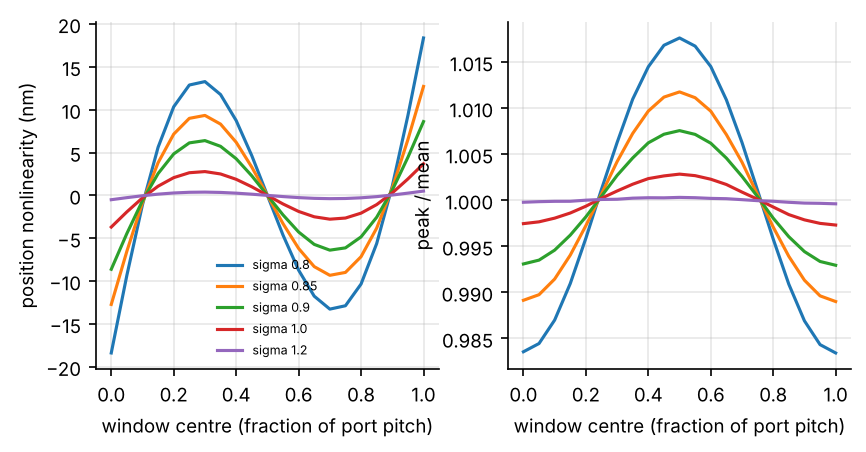
\includegraphics[width=0.75\linewidth]{m9_E_window.png}
\caption{Uncalibrated response of a sliding Gaussian window in the first (paraxial) route-E design, as the window centre moves across one port pitch, for window widths $\sigma = 0.8$ to 1.2 ports. Left: deviation of the spot position from a linear map. Right: peak intensity relative to its mean. 2D paraxial FPR with isolated port and arm modes, $N = 128$ ports at 2.0~\textmu m pitch (1.7~\textmu m wide), $R = 886$~\textmu m, 128 arms, emitter pitch 1.5~\textmu m, NA 0.5, 1064.4~nm. Both curves are periodic in the port pitch and are removed by a lookup table.}
\label{fig:engine-window}
\end{figure}

With 20 tweezers at random positions over $\pm60$~\textmu m and $\sigma = 0.9$ (calibrated), a tweezer moved by 0.1 to 4~\textmu m lands within 0.9~nm of its target with a peak change of at most 0.10\%, while the other 19 shift by at most 1.5~nm and 0.19\%. Removing a window leaves $8.9\times10^{-6}$ of the tweezer intensity at its site and changes the others by at most 0.08\%. The static peak spread of the 20 is 1.4\% with depth equalised by the tree. Two tweezers in quadrature at 2.5~\textmu m pull each other by 3.5~nm with a 0.16\% peak change, against 146~nm and 9.5\% in phase.

The cost lies in the actuators and their accuracy: 127 fast tunable splitters and 128 port phase shifters per chip. Because each tweezer is set by only about five ports, per-port errors average little. Per-port amplitude and phase errors of 0.3\%/3~mrad, 1\%/10~mrad and 3\%/30~mrad rms give position noise of 3.1, 9.4 and 28~nm and peak noise of 0.5, 1.9 and 5.6\%. Thus 10~nm needs about 1\% and 10~mrad, about 15 times tighter than the arm-side OPA (0.14~rad at $N = 64$, Sec.~\ref{sec:platform-opa}), and PZT hysteresis ([VALUE?]) must be corrected, for example by closed-loop calibration against on-chip taps. A moving tweezer is updated through the tree, so the staircase result applies: $\ge 200$~kHz updates at 1.2~mK, which PZT shifters (0.4~MHz~\cite{MONT}) meet and thermo-optic shifters (34~\textmu s rise) do not. The node settings follow in closed form from the desired port amplitudes, since each node splits in the ratio of the powers of its two subtrees, so an FPGA can compute them in real time. A tweezer is switched by ramping its window through the tree adiabatically ($\ge 100$~\textmu s), and its off-state is then set by the extinction of the tree nodes.

This last point decides the 894.6~nm engine. Raman gates act on atoms in static traps, and the addressed Raman leg must keep a fixed frequency relative to the global leg, so frequency tagging is unavailable at 894.6~nm. Route~E there would give steerable addressing with an off-state set by the tree nodes, rather than by a cascaded switch per beam. The switched-port star coupler of Sec.~\ref{sec:engine-star} therefore remains the addressing engine, and route~E the transport engine at 1064.4~nm.

\subsection{Design D1 by beam propagation}\label{sec:engine-D1}

The paraxial model above treats ports and arms as isolated and the FPR as aberration-free. Dense ports at 0.3~\textmu m gaps couple, and an AWG-type star coupler needs a full propagation design. Since the 400~nm film is uniform and fully etched, every guide and the slab share one vertical mode, and a lateral effective-index model carries the star-coupler physics. The plain effective-index model overestimates lateral confinement: its coupling lengths are 31 to 36\% short of the 3D vector-FEM values. We therefore calibrate the lateral core and cladding indices (1.8423 and 1.3551) to the vector-FEM effective indices of 0.6, 1.0 and 1.7~\textmu m guides (residuals $\le 4.3\times10^{-4}$) and to the coupling length of the dense ports (622 against 625~\textmu m); a held-out check on 1.4~\textmu m guides at 0.49~\textmu m gap agrees to 3\%, and narrow, widely spaced guides (off by 29\%) couple negligibly in the design. Propagation uses a 2D wide-angle (Pad\'e (1,1)) Crank-Nicolson beam-propagation method (BPM) with the TM-type lateral operator that matches the chip TE mode, all ports propagated together ($\Delta x = 0.04$~\textmu m, $\Delta z = 0.125$~\textmu m; capture converged to 0.5\%). On a reduced 8-port, 8-arm coupler, 2D FDTD and BPM agree in arm field with fidelity 0.997 (centre port) to 0.93 (edge port, rising to 0.981 at finer FDTD resolution) and in capture to 2 to 5\%, the residual being dominated by FDTD discretisation. For fast optimisation an exact-path Rayleigh-Sommerfeld model reproduces the full $128\times128$ BPM to within 1\% in capture and with arm-field fidelity 0.996 to 0.9996 (0.96 at the two extreme ports, where taper coupling matters); on the optimised design both give the same field-averaged efficiency to 0.6\%.

The propagation revealed two effects absent from the paraxial model. (i) The confocal coupler (ports on an arc of radius $R$) is aberrated: each off-axis port's arm phases deviate from a straight line by up to 1.3~rad peak-to-peak at the edge port (0.43~rad half-way out). Arm trims cannot remove this because it depends on the port. Placing the ports on an arc of radius $0.555R$, close to the Rowland circle, halves it over the field of use, and with 192 arms the worst residual is 0.08~rad rms; the different piston phase this gives each port is removed by static port trims. (ii) Neighbouring ports exchange light in the converging tapers. With fixed Gaussian windows this broadens the spot tails, and moving one of 20 tweezers then changes the others by up to 7~nm and 1.1\%. Both effects are linear and static, which the synthesis of Sec.~\ref{sec:engine-LS} exploits.

We then optimised the geometry for the field-averaged laser power per tweezer at equal depth, i.e.\ the harmonic mean of the peak intensity per unit port power over $|x| \le 60$~\textmu m, under the constraints of a neighbour intensity at 4~\textmu m of $\le 10^{-4}$, gaps $\ge 0.3$~\textmu m, and 128 ports (the fast actuators) fixed. The roll-off across the field has one origin on both sides of the chip, scan loss: the arms capture tilted light from off-axis ports, and the emitters radiate tilted beams, each with an element pattern that falls across its angular range. Two levers act on it (Fig.~\ref{fig:engine-opt}). Oversampling, i.e.\ more arms and emitters than ports, confines the ports to the central part of the arms' angular range and raises the edge capture from 0.44 to 0.54 with 192 arms. Arms and emitters carry only static trims in route~E, so this costs area and slow heaters, not fast actuators; 256 arms would add 7\% for 64 more trims and a 1.8~mm slab. Wider emitter facets narrow the element pattern and raise the relay transmission at the centre from 0.64 (0.6~\textmu m) to 0.84 (1.2~\textmu m at 1.5~\textmu m pitch). With 0.5~\textmu m gaps the transmission saturates near 0.74 to 0.76 for any pitch from 1.5 to 2.2~\textmu m, so the 0.3~\textmu m gap of the 1.2~\textmu m facet buys the last 10\%; its coupling length of 227~\textmu m limits the wide facet section to about 15~\textmu m. At the slab, the widest ports and arms (1.7~\textmu m at 2.0~\textmu m pitch) give a field-averaged efficiency of 0.261 against 0.18 to 0.24 for 1.2 to 1.5~\textmu m widths, because fill factor outweighs the slightly better angular acceptance of narrow arms. Narrowing the window from 0.9 to 0.85 ports gains 5\% but raises the neighbour intensity to $4.8\times10^{-5}$; we adopt least-squares synthesis with a 1.68~\textmu m target instead.

\begin{figure}[htbp]\centering
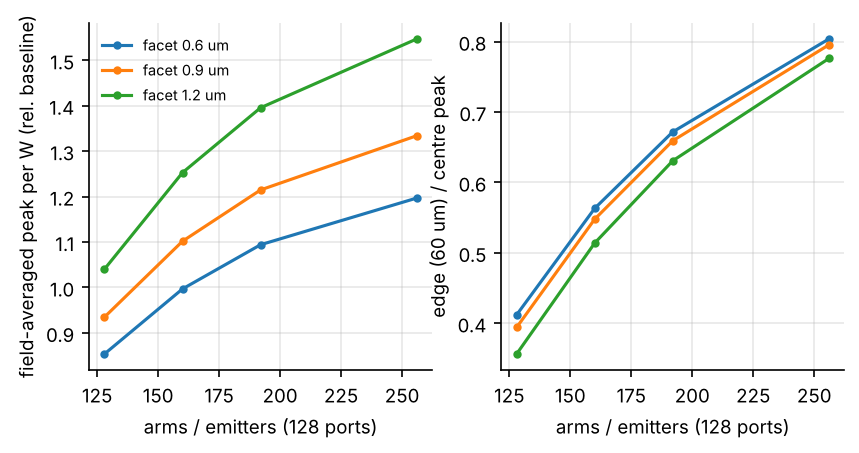
\includegraphics[width=0.75\linewidth]{m11_stage1.png}
\caption{Geometry optimisation of the route-E star coupler with 128 ports, against the number of arms and emitters, for emitter facets of 0.6, 0.9 and 1.2~\textmu m at 1.5~\textmu m pitch. Left: field-averaged peak intensity per unit port power (harmonic mean over $|x| \le 60$~\textmu m), relative to the confocal $128\times128$ design with 0.6~\textmu m facets. Right: peak at the field edge ($x = 60$~\textmu m) relative to the centre. Exact-path (Rayleigh-Sommerfeld) star-coupler model, ports on a Rowland-type arc of radius $0.555R$, ports and arms 1.7~\textmu m wide at 2.0~\textmu m pitch, Gaussian window $\sigma = 0.9$ ports, NA 0.5. D1 is the 192-arm, 1.2~\textmu m-facet point (gain 1.51, edge ratio 0.71).}
\label{fig:engine-opt}
\end{figure}

The resulting design D1 has 128 input ports and 192 arms, both 1.7~\textmu m wide at 2.0~\textmu m pitch at the slab (0.3~\textmu m gaps); a slab radius $R = 1329$~\textmu m; ports on an arc of radius $0.555R$ through the slab vertex, pointing at the arm-array centre; arms on an arc of radius $R$ with 30~\textmu m tapers to 0.6~\textmu m guides; 192 end-fire emitters at 1.5~\textmu m pitch with 1.2~\textmu m facets (facet taper $\le 15$~\textmu m); static phase trims on all arms and ports; and port amplitudes from least-squares synthesis.

\subsection{Least-squares port synthesis and residual errors}\label{sec:engine-LS}

Instead of fixed Gaussian windows, we compute the port amplitudes by least squares on the calibrated port-to-atom response, with the target spots as the objective. Because port coupling and aberration are linear and static, the synthesis removes them, at a cost of 1 to 2\% in efficiency, and it equalises depth over the field without a lookup table. Each update is one product with a precomputed $128\times n$ matrix. Table~\ref{tab:engine-D1} compares D1 with the first (confocal $128\times128$) design, both verified by BPM of the full structure with the calibrated effective-index model and least-squares synthesis.

\begin{table}[htbp]\centering\small
\caption{Simulated performance of the route-E engine: first confocal design against the optimised design D1 (full BPM, least-squares port synthesis, 20 tweezers over $\pm60$~\textmu m). Laser power uses facet $-0.37$~dB, 7-stage tunable tree $-0.39$~dB, 1~cm at 0.3~dB/cm and meta-objective transmission 0.7 (both assumed), and a 1.04~\textmu m Gaussian profile across the row; see the text for the revised value.}
\label{tab:engine-D1}
\begin{tabular}{@{}p{0.42\linewidth}cc@{}}
\toprule
quantity & first design & D1 \\
& ($128\times128$, confocal) & \\
\midrule
field-averaged peak per unit port power (relative) & 1.00 & 1.50 \\
edge (60~\textmu m) / centre peak & 0.52 & 0.70 \\
residual arm-phase aberration, worst port & $\le 1.3$~rad pk-pk & $\le 0.08$~rad rms \\
others' change when one of 20 moves by up to 4~\textmu m & $\le 3.5$~nm, $\le 0.12\%$ & $\le 3.5$~nm, $\le 0.11\%$ \\
residual at a switched-off site & $1.3\times10^{-6}$ & $1.6\times10^{-6}$ \\
static peak spread of 20 tweezers & 0.56\% & 0.52\% \\
spot FWHM along the row & 1.71~\textmu m & 1.71~\textmu m \\
laser power per 1.2~mK tweezer, field mean (fibre) & ${\sim}65$~mW & ${\sim}43$~mW \\
20 tweezers over $\pm60$~\textmu m & ${\sim}1.3$~W & ${\sim}0.86$~W \\
\bottomrule
\end{tabular}
\end{table}

Under full propagation with synthesis the others' displacement is up to 3.5~nm rather than the 1.5~nm of the paraxial windows (Sec.~\ref{sec:engine-E}), while the peak change, switch-off residual and peak spread are smaller. The per-port actuator accuracy, about 1\% and 10~mrad for 10~nm of position noise, is not relaxed by the synthesis and remains the main requirement on the hardware.

\subsection{Power per tweezer}\label{sec:engine-power}

The loss chain from fibre to atoms is the facet ($-0.37$~dB), the 7-stage tunable tree ($-0.39$~dB), 1~cm of propagation at 0.3~dB/cm (assumed, $-0.3$~dB), the simulated FPR, arms, emitters, slit and pupil, and a meta-objective transmission of 0.7 (assumed). In the first paraxial design a 1.2~mK tweezer needs 48~mW at the fibre at the field centre and 102~mW at the edge; equalising depth costs a mean factor of 1.34, so 20 tweezers spread over $\pm60$~\textmu m need about 1.3~W, and restricting operation to $\pm40$~\textmu m lowers the mean factor. D1 brings the field mean to about 43~mW (0.86~W for 20), a factor 1.5 in efficiency. However, both figures omit the cross axis and the emitter facet loss (about 21\% into air). With both included and a collimator glued to the facets, a 1.2~mK tweezer needs about 57~mW (\texttt{docs/stacked\_relay.md}, \texttt{docs/collimator.md}); this is the current value. For comparison, the switched-port star coupler, computed with the same Gaussian cross-axis profile, needs 33 to 43~mW per tweezer, and the proposal assumes 1.4~W for 21 tweezers.

\subsection{Limits}\label{sec:engine-limits}

The model is 2D with a calibrated effective index. The residual 3D effects, polarisation coupling at sidewalls and slab-edge scattering, are not computed, and the 3D excess loss of the dense-port FPR is open ([VALUE?]). Fabrication variation of the 0.3~\textmu m gaps and of the taper geometry has not been simulated; static errors are absorbed by the trims and the measured response matrix, but the arm phase errors after fabrication, which set the trim range, are not known ([VALUE?]). The relay and objective are scalar and aberration-free, so a meta-objective with a Strehl ratio of 0.8 adds a halo not included in the crosstalk figures. Steering is along one row; the second axis needs a second engine or an OPA-AOD hybrid. The hardware load of D1 is 255 fast actuators (127 tree splitters and 128 port phase shifters, which also carry the port trims) and 192 static arm trims, with PZT shifter footprint, hysteresis and long-term drift after closed-loop calibration still open ([VALUE?]). The procedure that measures the port-to-atom response on the device, on which the least-squares synthesis rests, has yet to be defined.
